\documentclass[12pt,a4paper,bibliography=totocnumbered,listof=totocnumbered]{scrartcl}
\usepackage[ngerman]{babel}
\usepackage[utf8]{inputenc}
\usepackage{amsmath}
\usepackage{amsfonts}
\usepackage{amssymb}
\usepackage{graphicx}
\usepackage{fancyhdr}
\usepackage{tabularx}
\usepackage{geometry}
\usepackage{setspace}
\usepackage[right]{eurosym}
\usepackage[printonlyused]{acronym}
\usepackage{subfig}
\usepackage{floatflt}
\usepackage[usenames,dvipsnames]{color}
\usepackage{colortbl}
\usepackage{paralist}
\usepackage{array}
\usepackage{titlesec}
\usepackage{parskip}
\usepackage[right]{eurosym}
\usepackage[subfigure,titles]{tocloft}
\usepackage[pdfpagelabels=true]{hyperref}

\usepackage{listings}
\lstset{basicstyle=\footnotesize, captionpos=b, breaklines=true, showstringspaces=false, tabsize=2, frame=lines, numbers=left, numberstyle=\tiny, xleftmargin=2em, framexleftmargin=2em}
\makeatletter
\def\l@lstlisting#1#2{\@dottedtocline{1}{0em}{1em}{\hspace{1,5em} Lst. #1}{#2}}
\makeatother

\geometry{a4paper, top=27mm, left=30mm, right=20mm, bottom=35mm, headsep=10mm, footskip=12mm}

\hypersetup{unicode=false, pdftoolbar=true, pdfmenubar=true, pdffitwindow=false, pdfstartview={FitH},
	pdftitle={Bachelorarbeit},
	pdfauthor={Fabian Wilms},
	pdfsubject={Bachelorarbeit},
	pdfcreator={\LaTeX\ with package \flqq hyperref\frqq},
	pdfproducer={pdfTeX \the\pdftexversion.\pdftexrevision},
	pdfkeywords={Bachelorarbeit},
	pdfnewwindow=true,
	colorlinks=true,linkcolor=black,citecolor=black,filecolor=magenta,urlcolor=black}
\pdfinfo{/CreationDate (D:20110620133321)}

\begin{document}

\titlespacing{\section}{0pt}{12pt plus 4pt minus 2pt}{-6pt plus 2pt minus 2pt}

% Kopf- und Fusszeile
\renewcommand{\sectionmark}[1]{\markright{#1}}
\renewcommand{\leftmark}{\rightmark}
\pagestyle{fancy}
\lhead{}
\chead{}
\rhead{\thesection\space\contentsname}
\lfoot{Generative Testerstellung für Microservice-Architekturen}
\cfoot{}
\rfoot{\ \linebreak Seite \thepage}
\renewcommand{\headrulewidth}{0.4pt}
\renewcommand{\footrulewidth}{0.4pt}

% Vorspann
\renewcommand{\thesection}{\Roman{section}}
\renewcommand{\theHsection}{\Roman{section}}
\pagenumbering{Roman}

% ----------------------------------------------------------------------------------------------------------
% Titelseite
% ----------------------------------------------------------------------------------------------------------
\thispagestyle{empty}
\begin{center}
	
\includegraphics[scale=0.5]{images/Hochschule_Muenchen_Logo.png}\\
	\vspace*{2cm}
	\Large
	\textbf{Fakultät für Informatik und Mathematik 07}\\
	\vspace*{2cm}
	\Huge
	\textbf{Bacheloararbeit}\\
	\vspace*{0.5cm}
	\large
	über das Thema\\
	\vspace*{1cm}
	\textbf{Generative Testerstellung für Microservice-Architekturenit}\\
	\vspace*{2cm}
	
	\vfill
	\normalsize
	\newcolumntype{x}[1]{>{\raggedleft\arraybackslash\hspace{0pt}}p{#1}}
	\begin{tabular}{x{6cm}p{7.5cm}}
		\rule{0mm}{5ex}\textbf{Autor:} & Fabian Wilms\newline holtkoet@hm.edu \\ 
		\rule{0mm}{5ex}\textbf{Prüfer:} & Prof. Dr. Ulrike Hammerschall \\ 
		\rule{0mm}{5ex}\textbf{Abgabedatum:} & xx.xx.2017 \\ 
	\end{tabular} 
\end{center}
\pagebreak

% ----------------------------------------------------------------------------------------------------------
% Abstract
% ----------------------------------------------------------------------------------------------------------
\setcounter{page}{1}
\onehalfspacing
\titlespacing{\section}{0pt}{12pt plus 4pt minus 2pt}{2pt plus 2pt minus 2pt}
\rhead{KURZFASSUNG}
\section{Kurzfassung}

Viele Softwareprojekte scheitern an fehlerhafter Kalkulation. Die Kosten werden meist viel zu gering angesetzt und sorgen für unzufriedene Kunden, geringe Erträge und fehlende Folgeaufträge. Doch warum ist das so?

Der größte Kostenfaktor sind Fehler im laufenden System. Diese Fehler zu beseitigen ist häufig eine große Herausforderung die viel Zeit, Personal und somit Geld kostet. Es gilt also, vor Auslieferung der Software eine entsprechende Qualität gewährleisten zu können.

Aus diesem Grund ist eine umfassende Testabdeckung ein sehr wichtiger Bestandteil in der Definition of Done der Landeshauptstadt München. Unit- und Integrations Tests sind fest in viele Entwicklungsprozesse integriert und finden besonders auch in agilen Entwicklerteams großen Zuspruch. Allerdings sind auch Tests finanzielle, wie auch zeitliche Kostenfaktoren.
Dennoch wird für Tests, trotz des Bewusstseins für die damit entstehenden Probleme, häufig viel zu wenig zeit eingeplant.

Um diesen problemen entgegen zu wirken wurde bei der LHM im vergangenen Jahr das Softwareprojekt Barrakuda entwickelt, welches anhand eines nach Domain Driven Design (DDD) aufgebauten Domänen-Modells Microservice Architekturen generieren kann. Die Idee: Software anhand von simplen Modellen generieren, um möglichst viel Zeit beim Entwickeln von "Boiler Plate"-Code einzsuparen, und die Software-Qualität nicht nur durch ersparte Entwicklungszeit, sondern auch durch homogene Projektstrukturen in allen generierten Systemen, und damit erhöhte Wartbarkeit, zu verbessern.

Im Rahmen dieser Bachelor-Arbeit soll die These geprüft werden, dass sich aus einem soclhen Modell genügend Informationen zum Testen eines Microservice-Frameworks extrahieren lassen, um eine ausreichende Testabdeckung für die generierten Services zu bieten.

Hierzu ist ein tieferes Verständnis der zu Generierung eingesetzten Sprache Barrakuda, welche von Martin Kurz in seiner Masterarbeit „Verbesserung des Softwareentwicklungsprozesses der Landeshauptstadt München durch modellgetriebene Softwareentwicklung“ entwickelt wurde, nötig. Diese wird in einem weiteren Abschnitt erklärt und anhand von Beispielen demonstriert. Um die Verbindung von Barrakuda zum DDD hervorzuheben, wird dies im weiteren Vorgehen näher beleuchtet.

Im zweiten Teilabschnitt werden dann die gängigsten Methoden und Praktiken, sowie Frameworks, die beim Testen von Microservice-Architekturen eingesetzt werden, identifiziert und weitere Anforderungsanalysen für diese durchgeführt, um die benötigte Bandbreite der generierten Tests abzugrenzen. Vorstellbare Testarten isnd Integrationstests, Unit-Tests und Smoke Tests.

Der letzte Schritt der Vorbereitung soll dann aus den zusammengetragenen Informationen festgestellen, für welches Framework ein generativer Ansatz zum Erstellen von Testfällen am sinnvollsten ist. Außerdem sollen eventuell benötigte Erweiterungen und/oder Änderungen von Barrakuda festgelegt werden, die für den generativen Ansatz von Nöten sind.

Im praktischen Teil der Arbeit werden dann zunächst einige Referenzimplementierungen umgesetzt, anhand derer im nächsten Teilschritt die Generierung der Tests, unter Zuhilfenahme von Barrakuda und den im vorherigen Teil festgelegten Änderungen, implementiert werden.

\vspace{-1,2em}
\titlespacing{\section}{0pt}{12pt plus 4pt minus 2pt}{-6pt plus 2pt minus 2pt}
\section*{Abstract}
Das ganze auf Englisch.
\pagebreak

% ----------------------------------------------------------------------------------------------------------
% Verzeichnisse
% ----------------------------------------------------------------------------------------------------------
% TODO Typ vor Nummer
\renewcommand{\cfttabpresnum}{Tab. }
\renewcommand{\cftfigpresnum}{Abb. }
\settowidth{\cfttabnumwidth}{Abb. 10\quad}
\settowidth{\cftfignumwidth}{Abb. 10\quad}

\titlespacing{\section}{0pt}{12pt plus 4pt minus 2pt}{2pt plus 2pt minus 2pt}
\singlespacing
\rhead{INHALTSVERZEICHNIS}
\renewcommand{\contentsname}{II Inhaltsverzeichnis}
\phantomsection
\addcontentsline{toc}{section}{\texorpdfstring{II \hspace{0.35em}Inhaltsverzeichnis}{Inhaltsverzeichnis}}
\addtocounter{section}{1}
\tableofcontents
\pagebreak
\rhead{VERZEICHNISSE}
\listoffigures
\pagebreak
\listoftables
%\pagebreak
\renewcommand{\lstlistlistingname}{Listing-Verzeichnis}
{\labelsep2cm\lstlistoflistings}
\pagebreak

% ----------------------------------------------------------------------------------------------------------
% Abkürzungen
% ----------------------------------------------------------------------------------------------------------
\section{Abkürzungsverzeichnis}
\begin{acronym}[OSGi] % längste Abkürzung steht in eckigen Klammern
	\setlength{\itemsep}{-\parsep} % geringerer Zeilenabstand
	\acro{DDD}{Domain-Driven Design}
	\acro{LHM}{Landeshauptstadt München}
\end{acronym}
\newpage

% ----------------------------------------------------------------------------------------------------------
% Inhalt
% ----------------------------------------------------------------------------------------------------------
% Abstände Überschrift
\titlespacing{\section}{0pt}{12pt plus 4pt minus 2pt}{-6pt plus 2pt minus 2pt}
\titlespacing{\subsection}{0pt}{12pt plus 4pt minus 2pt}{-6pt plus 2pt minus 2pt}
\titlespacing{\subsubsection}{0pt}{12pt plus 4pt minus 2pt}{-6pt plus 2pt minus 2pt}

% Kopfzeile
\renewcommand{\sectionmark}[1]{\markright{#1}}
\renewcommand{\subsectionmark}[1]{}
\renewcommand{\subsubsectionmark}[1]{}
\lhead{Kapitel \thesection}
\rhead{\rightmark}

\onehalfspacing
\renewcommand{\thesection}{\arabic{section}}
\renewcommand{\theHsection}{\arabic{section}}
\setcounter{section}{0}
\pagenumbering{arabic}
\setcounter{page}{1}

% ----------------------------------------------------------------------------------------------------------
% Einleitung
% ----------------------------------------------------------------------------------------------------------
\section{Einleitung}
Dieses Kapitel enthält Beispiele zum Einfügen von Abbildungen, Tabellen, etc.

\subsection{Problem}
Zum Einfügen eines Bildes, siehe Abbildung \ref{fig:osgi}, wird die \textit{minipage}-Umgebung genutzt, da die Bilder so gut positioniert werden können.

\vspace{1em}
\begin{minipage}{\linewidth}
	\centering
	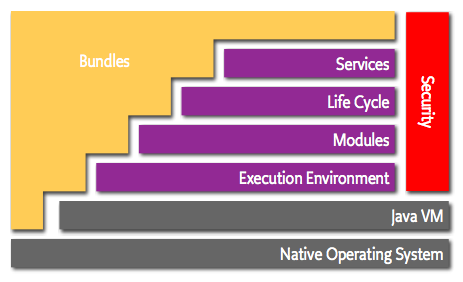
\includegraphics[width=0.7\linewidth]{images/layering-osgi.png}
	\captionof{figure}[OSGi Architektur]{OSGi Architektur\footnotemark }
	\label{fig:osgi}
\end{minipage}
\footnotetext{Quelle: \url{http://www.osgi.org/Technology/WhatIsOSGi}}

% ----------------------------------------------------------------------------------------------------------
% Kapitel
% ----------------------------------------------------------------------------------------------------------
\section{Kapitel}
Lorem ipsum dolor sit amet.

\subsection{Unterkapitel}
Lorem ipsum dolor sit amet, consetetur sadipscing elitr, sed diam nonumy eirmod tempor invidunt ut labore et dolore magna aliquyam erat, sed diam voluptua. At vero eos et accusam et justo duo dolores et ea rebum. Stet clita kasd gubergren, no sea takimata sanctus est Lorem ipsum dolor sit amet. Lorem ipsum dolor sit amet, consetetur sadipscing elitr, sed diam nonumy eirmod tempor invidunt ut labore et dolore magna aliquyam erat, sed diam voluptua. At vero eos et accusam et justo duo dolores et ea rebum. Stet clita kasd gubergren, no sea takimata sanctus est Lorem ipsum dolor sit amet.

\subsection{Unterkapitel}
Lorem ipsum dolor sit amet, consetetur sadipscing elitr, sed diam nonumy eirmod tempor invidunt ut labore et dolore magna aliquyam erat, sed diam voluptua. At vero eos et accusam et justo duo dolores et ea rebum. Stet clita kasd gubergren, no sea takimata sanctus est Lorem ipsum dolor sit amet. Lorem ipsum dolor sit amet, consetetur sadipscing elitr, sed diam nonumy eirmod tempor invidunt ut labore et dolore magna aliquyam erat, sed diam voluptua. At vero eos et accusam et justo duo dolores et ea rebum. Stet clita kasd gubergren, no sea takimata sanctus est Lorem ipsum dolor sit amet.
\pagebreak

% ----------------------------------------------------------------------------------------------------------
% Literatur
% ----------------------------------------------------------------------------------------------------------
\renewcommand\refname{Quellenverzeichnis}
\bibliographystyle{bibstyle}
\bibliography{bibfile}
\pagebreak

% ----------------------------------------------------------------------------------------------------------
% Anhang
% ----------------------------------------------------------------------------------------------------------
\pagenumbering{Roman}
\setcounter{page}{1}
\lhead{Anhang \thesection}

\begin{appendix}
\section*{Anhang}
\phantomsection
\addcontentsline{toc}{section}{Anhang}
\addtocontents{toc}{\vspace{-0.5em}}

\section{Code-Fragmente}
Viel Beispiel-Code

\end{appendix}

\end{document}
